\documentclass[pdf,sprung,slideColor,nocolorBG]{beamer}
%
%\documentclass[hyperref={pdfpagelabels=false}]{beamer}
\mode<presentation>

\newenvironment{colortheme}[1]{
\def\ProvidesPackageRCS $##1${\relax}
\renewcommand{\ProcessOptions}{\relax}
\makeatletter
\input beamercolortheme#1.sty
\makeatother
}{}

\let\Tiny=\tiny
\usetheme{Adelaide}
\usefonttheme[stillsansseriftext]{serif}
\setbeamerfont{structure}{series=\bfseries}
\setbeamertemplate{frametitle}[default][center]
\usepackage{svg}
\svgsetup{}
\usepackage[figurename={}]{caption}
\usepackage[latin1]{inputenc}
%\usepackage{amsmath}   %needed for \begin{align}... \end{align} environment
\usepackage{amsfonts}
\usepackage{amssymb}
\usepackage{amscd}
\usepackage[all]{xy}
\usepackage{xcolor}
\usepackage{enumerate}
%
\newcommand{\slidecite}[1]{\tiny{(#1)}\normalsize{}}
\newcommand{\smallcite}[1]{\small{(#1)}\normalsize{}}

\newcommand{\mb}[1]{\mathbb{#1}}
\newcommand{\mf}[1]{\mathbf{#1}}
\newcommand{\Emph}[1]{\emph{\textcolor{blue}{#1}}}

\newcommand{\abs}[1]{\left| #1 \right|}
\newcommand{\norm}[1]{\left\| #1 \right\|}
\newcommand{\To}{\rightarrow}

\newcommand{\Cay}[1]{\operatorname{Cay}\left(#1\right)}
\newcommand{\Clique}[1]{\omega\left(#1\right)}
\newcommand{\dual}[1]{\widetilde{#1}}
\newcommand{\support}[1]{\operatorname{supp}\left(#1\right)}
\newcommand{\weight}[1]{\operatorname{wt}\left(#1\right)}
\newcommand{\weightclass}[1]{\operatorname{wc}\left(#1\right)}

\newcommand{\G}{\mb{G}}
\newcommand{\R}{\mb{R}}
\newcommand{\Z}{\mb{Z}}
%\newtheorem{Definition}{Definition}
\newtheorem{Question}{Question}
\newtheorem{Conjecture}{Conjecture}

\title{Big data in combinatorics: is it FAIR?}
\author{Paul Leopardi}

\date{For 42 ACCMCC UNSW Sydney 2019}

\institute{Australian National University.}
\titlegraphic{
%\includegraphics[angle=0,width=10mm]{../../common/beamer-anu-colourlogo.png}
%\includegraphics[angle=0,width=20mm]{../../common/carma_logo.jpg}
}
\begin{document}

\frame{\titlepage}
\begin{frame}
\frametitle{Acknowledgements}
\begin{center}
~
 
Katja Ber\u{c}i\u{c}, Michael Kohlhase, Nicolas Thiery.
 
~

Australian National University.

~

SageMath, Bliss, Nauty.

~

National Computational Infrastructure.
\end{center}
\end{frame}

\begin{frame}
\frametitle{Overview}
%\begin{center}
\begin{itemize}
\item
FAIR data principles

~

\item
The OpenDreamKit project

~

\item
Some datasets

~

\item
Work in progress

\end{itemize}
 
%\end{center}
\end{frame}

\section{FAIR}
\begin{colortheme}{jubata}
\begin{frame}
\frametitle{The FAIR data principles}
%\begin{center}
In 2014, a Lorentz Center (Leiden) workshop began formulating the FAIR 
Data Principles for research data.
These principles were elaborated over the following two years.

~

FAIR stand for Findable, Accessible, Interoperable, Reusable

~

\slidecite{Aalbersberg et al. 2014, Wilkinson et al. 2016}
\end{frame}
\begin{frame}
\frametitle{To be Findable}
%\begin{center}
\begin{description}
 \item[F1] (meta)data are assigned a globally unique and persistent identifier
 \item[F2] data are described with rich metadata (defined by R1)
 \item[F3] metadata clearly and explicitly include the identifier of the data it describes
 \item[F4] (meta)data are registered or indexed in a searchable resource
\end{description}

~

\slidecite{Wilkinson et al. 2016}
\end{frame}
\begin{frame}
\frametitle{To be Accessible}
%\begin{center}
\begin{description}
 \item[A1] (meta)data are retrievable by their identifier using a standardized communications protocol
 \item[A1.1] the protocol is open, free, and universally implementable
 \item[A1.2] the protocol allows for an authentication and authorization procedure, where necessary
 \item[A2] metadata are accessible, even when the data are no longer available
\end{description}

~

\slidecite{Wilkinson et al. 2016}
\end{frame}
\begin{frame}
\frametitle{To be Interoperable}
%\begin{center}
\begin{description}
 \item[I1] (meta)data use a formal, accessible, shared, and broadly applicable language for knowledge representation.
 \item[I2] (meta)data use vocabularies that follow FAIR principles
 \item[I3] (meta)data include qualified references to other (meta)data
\end{description}

~

\slidecite{Wilkinson et al. 2016}
\end{frame}
\begin{frame}
\frametitle{To be Reusable}
%\begin{center}
\begin{description}
 \item[R1] meta(data) are richly described with a plurality of accurate and relevant attributes
 \item[R1.1] (meta)data are released with a clear and accessible data usage license
 \item[R1.2] (meta)data are associated with detailed provenance
 \item[R1.3] (meta)data meet domain-relevant community standards

\end{description}

~

\slidecite{Wilkinson et al. 2016}
\end{frame}
\begin{frame}
\frametitle{The FAIR data principles in Australasia}
%\begin{center}

\begin{itemize}
 \item 
Australian FAIR access working group

~

\footnotesize
 F.A.I.R. Access Policy Statement


 ``By 2020, Australian publicly funded researchers and research organisations will have in place policies, standards and practices to:
\begin{enumerate}
 \item Make publicly funded research outputs findable, accessible, interoperable and reusable \ldots''
\end{enumerate}
\normalsize

~

\item
Strategic Science Investment Fund (New Zealand)

~

\footnotesize
New Zealand Data Science Research Programmes Call for Proposals


``Describe the excellence of your team by telling us: \ldots
How you will access, analyse and share data, via
appropriate systems and tools, including implementation of
the FAIR data principles for scientific data management and
stewardship. \ldots''

\end{itemize}

~

\slidecite{https://www.fair-access.net.au/; https://www.mbie.govt.nz/}
\end{frame}
\section{OpenDreamKit}
\begin{frame}
\frametitle{The OpenDreamKit project}

The EU funded OpenDreamKit project (2015-2019) included a census of mathematical data sets, 
and the development of prototypical semantic infrastructure for the FAIR sharing of such data sets.

~

This used the idea of ``Deep FAIR'': FAIR sharing at the level of mathematical objects.

~

\slidecite{OpenDreamKit Project 2015-2019}
\end{frame}
\begin{frame}
\frametitle{Semantics of concrete data: an example}

Graphs, up to isomorphism can be stored using a canonical labelling in Graph6 format.

~

Different Graph6 strings represent non-isomorphic graphs, 
\emph{as long as the same canonical labelling algorithm is used}.

~

In SageMath 8.6, the \texttt{"bliss"} and \texttt{"sage"} algorithms yield \emph{different}
canonical labels for the same graph.

~

Thus some sort of semantic metadata needs to be stored in long term graph databases,
to avoid having to canonically label again.

~

\slidecite{SageMath 2019}
\end{frame}
\begin{frame}
\frametitle{Semantic infrastructure in OpenDreamKit}

Math in the Middle, MMT
\begin{center}
\includegraphics[width=80mm]{MitM.png}
\end{center}

\slidecite{OpenDreamKit Project 2015-2019; Kohlhase 2018 }
\end{frame}
\begin{frame}
\frametitle{Semantic infrastructure in OpenDreamKit}

Math in the Middle, MMT, virtual theories
\begin{center}
\includesvg[width=40mm]{use-cases-lmfdb-mitm.svg}
\hspace{10mm}
\includesvg[width=50mm]{use-cases-lmfdb-mediator.svg}
\end{center}

\slidecite{OpenDreamKit Project 2015-2019}
\end{frame}
\begin{frame}
\frametitle{The FAIRmat project proposal}

The FAIRmat project was intended to be a follow-on from the OpenDreamKit project,
concentrating on the furter development of FAIR infrastructure for mathematical software
and datasets, within the European Open Research Cloud.

~

The project was intended to begin in 2020, but was not funded.

~

\slidecite{FAIRmat Project Proposal, Kohlhase 2019}
\end{frame}
\end{colortheme}
\section{Datasets}

\subsection{Precedents}

\begin{colortheme}{jubata}

\begin{frame}
\frametitle{Datasets of bent functions}
\begin{itemize}
 \item
Langevin's lists of partial spread bent functions.

~

 \begin{itemize}
  \item
Flat text files.
  \item
Encoded by algebraic normal form.
 \end{itemize}

~

 \item
Langevin's ``Classification of Boolean Quartics Forms in eight Variables.''

~

 \begin{itemize}
  \item
Flat text files.
  \item
Encoded by algebraic normal form.
  \item
Does not explicitly enumerate bent functions or their equivalence classes.
 \end{itemize}

\end{itemize}

\slidecite{Langevin 2010; Langevin 2008}
\end{frame}

\begin{frame}
\frametitle{Databases of strongly regular graphs}
\begin{itemize}
 \item
Spence's lists of strongly regular graphs on at most 64 vertices.
 \begin{itemize}
  \item
Exhaustive lists of non-isomorphic graphs for some tuples of feasible parameters.
  \item
Flat text files.
 \end{itemize}

~

 \item
Brouwer's database of parameters of strongly regular graphs.

~

 \item
Cohen and Pasechnik's Sage implementation of Brouwer's database, with constructions.
 \begin{itemize}
  \item
Example for each tuple of feasible parameters, if known.
  \item
Sage interface.
 \end{itemize}
\end{itemize}
\slidecite{Spence 1995-2006; Brouwer 2008-2017; Cohen and Pasechnik 2016-2017}
\end{frame}

\begin{frame}
\frametitle{Other recent mathematical datasets}
\begin{itemize}
 \item
House of Graphs: a databse of interesting graphs
 \begin{itemize}
  \item
``\ldots The key principle is to have a searchable database and offer–next to complete lists of some graph classes -- also a list of special graphs that have already turned out to be interesting and relevant in the study of graph theoretic problems or as counterexamples to conjectures.''
  \item
Web-based interface.
 \end{itemize}

~

 \item
LMFDB - The L-functions and modular forms database
 \begin{itemize}
  \item
``The LMFDB is an extensive database of mathematical objects arising in Number Theory.''
  \item
Based on MongoDB and Python.
  \item
Web-based and Sage interfaces.
 \end{itemize}
\end{itemize}
\slidecite{Brinkmann et al. 2013; The LMFDB Collaboration 2007-2017}
\end{frame}

\end{colortheme}

\subsection{Prototype databases}

\begin{colortheme}{jubata}

\begin{frame}
\frametitle{Bent function Cayley graph databases}
Three prototype relational databases, using SQLite:

\begin{itemize}
 \item\normalsize{}
Bent functions in 6 dimensions.
 \begin{itemize}
  \item\footnotesize{}
Database of 11 strongly regular graphs from 4 ET classes.
  \item\footnotesize{}
Database size 780 KB.
 \end{itemize}

 \item\normalsize{}
Bent functions in 8 dimensions, up to degree 3.
 \begin{itemize}
  \item\footnotesize{}
Database of 55 strongly regular graphs from 9 ET classes.
  \item\footnotesize{}
Database size 65 MB.
 \end{itemize}

 \item\normalsize{}
Bent functions from the 8 S-boxes of CAST-128.
 \begin{itemize}
  \item\footnotesize{}
Database of more than \Emph{32 million} ($32\,914\,496$) strongly regular graphs from 256 ET classes and their duals.
  \item\footnotesize{}
Database size \Emph{195 GB}.
 \end{itemize}
\end{itemize}
\normalsize{}

Flat directories of SageMath sobj files:

\footnotesize
About \Emph{2 billion} strongly regular graphs from 
the 14 758 ET classes of partial spread bent functions in 8 dimensions and their duals.
\Emph{Over 6 TB} total size.
\normalsize

\end{frame}

\begin{frame}
\frametitle{Schema for Cayley graph databases}
\begin{figure}
\centering
\begin{minipage}{\textwidth}
  \centering
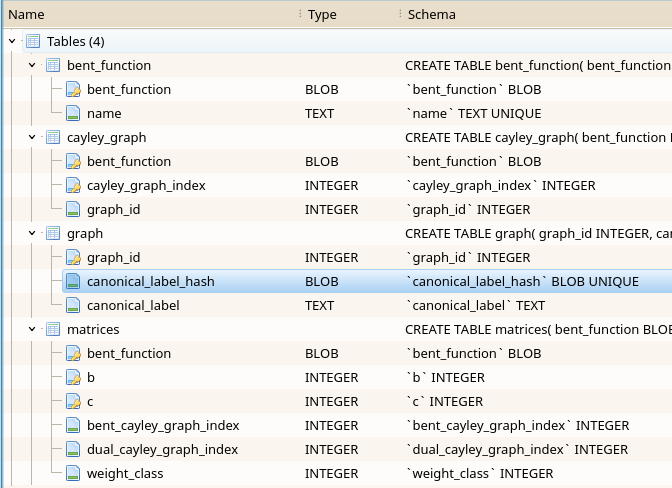
\includegraphics[width=.75\linewidth]{../graphics/Classification-schema-SQLite.png}
  \captionof{figure}{Database schema for SQLite version of the classification database.}
  \label{fig:Classification_schema_SQLite}
\end{minipage}%
\end{figure}
\end{frame}


\begin{frame}
\frametitle{Possible use case: Roberson's classification of strongly regular graphs}

Roberson recently proved that all strongly regular graphs are cores or have complete cores, proposing four types, A, B, C, X according to clique number and chromatic number.

~

Question: for each dimension of bent functions, determine the number of strongly regular Cayley graphs of each type.

~

\slidecite{Roberson 2019}
\end{frame}

\end{colortheme}

\subsection{Source code}

\begin{colortheme}{jubata}

\begin{frame}[fragile]
\frametitle{Bent function Cayley graph Sage code}
~

CoCalc: Public worksheets, Sage and Python source code

\begin{verbatim}
http://tinyurl.com/Boolean-Cayley-graphs
\end{verbatim}

~

GitHub: Sage and Python source code

\begin{verbatim}
https://github.com/penguian/Boolean-Cayley-graphs
\end{verbatim}

~

PyPI: Installable Python package


\begin{verbatim}
https://pypi.org/project/boolean-cayley-graphs/
\end{verbatim}

~

SourceForge: Documentation of Python modules

\begin{verbatim}
https://boolean-cayley-graphs.sourceforge.io/
\end{verbatim}

\end{frame}

\end{colortheme}

\subsection{Prospects}

\begin{colortheme}{jubata}

\begin{frame}[fragile]
\frametitle{Possible next steps}

\begin{itemize}
 \item
Rewrite and resubmit ``Classifying bent functions by their Cayley graphs.''

~

 \item
Develop a RESTful API for the bent function Cayley graph databases.

~

 \item
Develop semantic interfaces using Math-in-the-Middle, and other OpenDreamKit services.

~

 \item
Arrange for hosting. EUDAT? Australian Research Data Commons?

~

 \item
Scale up to the partial spread bent functions?
\end{itemize}

\end{frame}

\end{colortheme}

\end{document}
